% !TEX root = ./master.tex

\subsection{Le son et l'écoute}

Lors d'un concert, si nous pouvions visualiser les sons qui
s'échappent de l'orchestre, ce serait un chatoiement de cercles qui se
répandraient tout autour de nous, comme
la propagation des
ronds dans l'eau suite à un ébranlement de sa surface.
Les molécules d'air en contact avec la source sonore se déplacent et
créent une vibration. \autocite[p. 183]{bencivelli:pourquoi,}.


Le son peut être déterminé par différents paramètres
physiologiques et psychologiques.
Il est défini très précisément par un ensemble d'unités physiques chiffrées
: les décibels  et les hertz.\footnote{Cf. Annexe: Le son et sa
  définition.}
Lorsque nous serons au chapitre concernant l'étude clinique,
ces quelques informations mises en annexe seront pertinentes lors de la lecture des tests.
%Si la
%musicothérapie a un impact certain sur la façon d'écouter en
%entraînant sa
%modification, peut-elle être  démontrée et démontrable, \textsl{objectivée},
%simplement sous la forme d'un test, comme saisie par
%l'\oe il neutre de l'objectif d'un appareil
%photographique?

%Cette hypothèse formulée va être donc l'objet de notre étude qui
%débutera par la notion d'écoute que nous allons revisiter.



\subsection{Ecouter et entendre}
\paragraph{Ecouter ou entendre : une différence}

La définition du verbe `entendre' et du verbe `écouter'
\autocite[pp. 361--385]{hachette:dictionnaire} nous paraît opportune
en raison de la confusion courante des deux termes :
\begin{description}
\item[Entendre] c'est  percevoir des sons, saisir par l'ouïe.
\item[Ecouter] a trois sens:
\begin{enumerate}
	\item prêter l'oreille à; s'appliquer à entendre;
	\item prêter attention à l'avis de quelqu'un, suivre un avis;
	\item \emph{fig} suivre une impulsion,	une inspiration.
\end{enumerate}
\end{description}


Par les sources étymologiques du
terme `écouter' ,
 sa racine sanskrite \emph{ ``avih'' } se traduit par
 \emph{``évidence'' , ``connaissance'', ``discernement''}. Puis, en ancien
 français, ce mot a donné \textit{``oüir''} signifiant aussi bien \textit{``entendre''} ,
\textbf{`` écouter'' } que \textit{``comprendre''} \autocite {etymologieWeb}
 Est-ce la raison
pour laquelle il subsiste toujours un amalgame
sur le sens de ce verbe?
Selon Didier
Colin \autocite {colin2015}, cette faculté
permet non seulement d'écouter et de comprendre avec plus d'attention
mais aussi de percevoir des sons et peut même, être doué de
\textit{``clairaudience'}'.
En définitive, \emph{entendre} est une attitude passive par rapport au monde sonore
qui nous entoure. Nous recevons les sons sans les interpréter, sans
effort, étant une action involontaire, non
sélective, et plus simplement:  elle
\begin{quote}
	<<\,suppose un son (physique), une oreille
	pour le capter, un système nerveux pour le recevoir.\,>>\autocite[p. 2, ch . 1]{auriol:cle}
 \end{quote}
 Tandis qu'\textit{écouter}
\begin{quote}
	<<\,est un
	processus actif supposant préférences et répulsions pour tel son ou
	telle séquence sonore.\,>>\autocite[p. 2, ch . 1]{auriol:cle}

\end{quote}
Entendre et écouter sont donc  «\,deux
fonctions essentiellement distinctes bien qu'évoluant apparemment sur
des terrains iden\-ti\-ques\,>>
% ancien texte {\textbf{site internet: http: auriol.free.fr} Extrait de l'entretien réalisé par
%	Bernard Auriol avec Alfred Tomatis, 1973.}.
[\dots] avec «\,l'é\-lé\-ment cons\-cient, facteur essentiel sur lequel repose toute la
différence entre ces deux activités\,». \autocite[]{tomatis_oreille_1991}
\begin{quote}

	<<[\ldots] \emph{Entendre, c'est en quelque sorte subir
		un son} ou un message qui nous est adressé. \emph{Ecouter, c'est désirer appréhender ce son} ou ce message [\ldots]>>
	\autocite{tomatis:education}.
\end{quote}
Selon B. Auriol \autocite[18] {auriol:cle} et Tomatis \autocite[52]
{tomatis:loreille}, l\textbf{'écoute} est un `` éveil auditif''  défini avec au
minimum trois
fréquences simultanées (dans le sens esthétique). Il s'agit donc d'un phénomène
complexe avec la corrélation d'axes
linéaires (notion temporelle) et verticales (notion spatiale), doublée d'une
dimension psychologique.
En effet, si \enquote{\emph{Je suis la musique que je fais ou écoute}}\autocite{viret:b}, \textbf{écouter} implique une conscience pour s'actualiser dans le sujet.
Elle est une opération
qui suppose une participation active dans le choix du message
ou dans la sélection d'une voix. Elle  implique la volonté,
\pdfmargincomment[color=green]{Bien!}
permet une forme de décodage:
si nous nous trouvons dans un ambiance sonore à fort volume, pour
parvenir à lire, nous
ferons abstraction des bruits environnants tout en en ayant
conscience, parvenant à nous en extraire pour focaliser notre
attention sur cette lecture. Nous parvenons à couper les sons parasites, à nous en abstraire pour
nous concentrer uniquement sur les plus  pertinents. Et ceci se fait grâce à cette capacité si importante
d'\textbf{écoute} en connection avec notre cerveau.
%Dans un milieu sonore important,
% bruyant, comme un café, lorsque nous lisons attentivement, nous faisons abstraction
%des bruits environnants; en soi, nous les entendons parfaitement mais nous n'y
%prêtons pas attention.
Puisant encore davantage dans  la racine de ce mot, ``écouter'' signifirait
aussi \emph{partager}, ayant tout son sens lors d'un dialogue ou
avec la voix (supposée, imaginée) de  l'écrivain qui
 chante à travers un livre avec celle, intérieure, du lecteur.
 % phénomène se réalise avec un livre qui transmet et partage des
  %connaissances. L'écoute permet donc la communication, sous-entend le
 % plus souvent la présence d'un être en vis-à-vis et nécessite de la
 % concentration. Il faut cette volonté inclue dans celle-ci  pour
 % comprendre et rentrer en contact avec la voix de  l'écrivain qui
 % chante dans le texte avec celle, intérieure, du lecteur.


  \textbf{Ecouter} se base ainsi certes sur une stimulation prenant sa source à
l'extérieur mais devant être \textbf{ intérieurement et intentionnellement
	recherchée}.




      \paragraph{Ecoute musicothérapeutique}


Par extrapolation, nous pouvons aussi différencier les différents types d'écoute. D'après Edith Lecourt \autocite[ch. 10 <<\,De l'écoute verbale à l'écoute musicale\,>>, p. 182.]{lecourt:decouvrir}
 on en distingue plusieurs : l'écoute verbale, musicale, plurivocale et multiple.
 L'analyse musicale qui permet la différenciation d'une voix d'un ensemble polyphonique est appelée \emph{plurivocale}. Celle qui est multiple n'est pas analytique  mais
 \begin{quote}
 	 [\ldots] \textit{ouvre une disponibilité, met en suspens les grilles verbale et musicale} [\ldots] \emph{pour parcourir le vécu sonoro-affectif}\autocite[p. 183]{lecourt:decouvrir}.
 \end{quote}
 Employée en musicothérapie, elle la nomme la technique de la  \emph{communication sonore} qui peut apporter
 <<\,des ouvertures sur l'analyse des niveaux plus archaïques de l'organisation mentale\,>>\autocite[p. 154]{lecourt:decouvrir}.
 Par l'expérience musicale en groupe, il peut y avoir un moment
 particulier, de ``grâce"  nommé ``le concept d'illusion groupale",
 l'illusion d'une unité absolue, comme un seul corps \autocite{anzieu:groupal}.

\emph{Ecouter} implique donc les notions de \emph{son} et
d'\emph{oreille}. Nous allons dans un premier temps approfondir  la
définition du son dont les caractéristiques physiques seront mis en
annexes et il en sera de même pour l'oreille et les détails
d'anatomie.\footnote{Annexe 1.: Son et Oreille}
La compréhension de ces aspects que sont le son et l'oreille nous
permettrons de mieux situer notre travail et les hypothèses y afférentes.








\paragraph{Ecoute objective ou subjective?}

Nous avons tous,
selon les manuels d'anatomie, la même
oreille, du moins nous pouvons reconnaître une analogie de structure. Nous devrions donc entendre et écouter la même chose
lors d'une même information diffusée tout comme le fait un enregistreur avec un micro. Pourtant il n'y a pas d'écoute \emph{passive}. Chacun n'entend pas de la même manière les mêmes
informations, chacun trie et fait son propre choix selon la fonction
d'écoute élaborée depuis l'enfance. Cette fonction sélectionne très
rapidement les mots pour être intelligible, pour se faire
comprendre. Nous rejoignons l'idée de Tomatis lorsqu'il affirme que
\textit{"L'oreille a un psychisme"} , car tout un chacun entend ce qu'il veut bien
entendre \autocite{tomatis_oreille_1998}.
Nous transformons notre écoute selon nos attentes.
Allant dans le même sens, cet
article d'une
étude franco-américaine scientifique
\autocite{fritz_stradivarius} au sujet des célèbres violons
Stradivarius: faite avec un protocole
d'écoutes en aveugle avec
des violonistes professionnels et en parallèle avec un public (caché
derrière un rideau), elle démontre que le mythe de la suprématie
de ces instruments extrêmement chers tombe au profit d'instruments
neufs.
Le cerveau
transforme les informations reçues selon nos attentes et joue un
rôle majeur dans notre perception.
\autocite{lemonde.fr:stradivarius}.
%
%\footnote{\href{http://www.lemonde.fr/culture/article/2014/04/10/le-stradivarius-detrone-par-les-violons-modernes\_4398681\_3246.html}{LeMonde.fr}.}.
\autocite[p. 43]{roque:lecoute}


Qu'en est-il chez des patients venant consulter en thérapie et souvent
en souffrance émotionnelle? Sont-elles dues à des situations
insupportables qui
ordonnent à notre cerveau de se protéger en obscurcissant la
perception sonore?  Ne plus écouter certains
sons permettrait-il en quelque sorte d'échapper à la souffrance et de faire une
pause dans la douleur. Nous avons le droit et c'est un réflexe de
survie de ne pas vouloir assister à une scène insupportable et de détourner
notre regard. Nous pourrions supposer qu'il en est de même pour l'oreille ne voulant plus capter
certains sons.
Freud mettait déjà en évidence le phénomène de la
\textbf{sélectivité }comme ``mécanisme de défense'' \autocite{ Freud}.
Vouloir voir, c'est viser, vouloir entendre, c'est
    écouter.
L'\oe il regarde par la rétine et  vise, sous l'ordre du
cerveau, avec la macula. Dans la même idée, par l'écoute, nous avons
l'oreille et la cochlée (partie interne de l'oreille) qui permet
l'analyse des sons. Vouloir entendre dans le but d'écouter est comparable  à
la visée de l'\oe il lorsque l'on veut collecter une
information.
 En définitive, l'audition est la capacité perceptive du système auditif et l'écoute, c'est ce qu'on en fait.


\subsection{La perception des sons et l'existence de troubles
  émotionnels}


Conformément à l'idée que l'oreille nécessite d'être sollicitée pour
énergiser le corps et le cerveau en vue d'un épanouissement, la
capture d'un très haut nombre de stimulations par seconde agit
sur la \gls{réticulée}\footnote {Cf. Glossaire.},
%%%(Cf. Glossaire)
comme prouvé par d'incessantes recherches scientifiques actuelles,
confirmant la très grande complexité de notre cerveau.








\paragraph{ L'écoute dans le rapport
  musique-cerveau}

Depuis la plus haute Antiquité,  la reconnaissance de
l'impact de la musique sur l'émotion est actuellement confirmée par
des approches récentes, dont A.Damasio  \autocite {damasio:lautre},
%\footnote {{L'erreur de Descartes}, Antonio Damasio, Paris,  Ed.Odile Jacob, 1997},
qui souligne l'indispensabilité de l'\textbf{émotion}
sur l'intelligence   ---     \textbf{intelligence émotionnelle et intelligence
  cognitive} ---.
En outre, les approches neuro-psychologiques sur les \textit{agnosies
  auditives} \autocite[ pp. 205--216]{seron.baron.ea:neuropsychologie},
sur la perception distincte des émotions de la musique
\autocite[pp. 223--224]{platel_neuropsychology_2002},
sur l'apport de Bigand E. \autocite[Ch. 3
p. 35, "Vous avez l'oreille musicale"]{bigand:cerveau} \footnote {Bigand E., chercheur, professeur
de psychologie cognitive à l'Université 2013 }soutenant le
manque de fonction biologique précise de la musique,
et sur la
découverte du rôle mimétique des\textit{ neurones miroir }( ``troisième''
cerveau) de Rizzolati G. (1990)
\autocite[118--119]{van_eersel_cerveau},
%\footnote{"Notre cerveau n'a pas fini de nous étonner", Entretien
%avec Jean-MichelOughourlian, Ed. Albin Michel, Le Livre de Poche 2012}
toutes ces recherches nous permettent de maintenir et
appuyer
la fonction thérapeutique de la musique.











Quant au lien entre audition et troubles de l'humeur, comme souffrent
les patients testés, d'autres perspectives
récentes mettent en lumière les évaluations de ces dernières comme les
approches de Yowell (1995) \footnote{Yovell
  Y., Sackeim, H.A., Epstein, D.G., Prudlic, J., Devanand, D.P.,
  McElhiney, M.C., Settembrino, J.M. Bruder, G.E., 1995. Hearing loss
  asymmetry in major depression. J. Neuropsychitr. Clin. Neurosci. 7,
  82--89.} Millot and Brand (2001) et
Canbeyli (2010) \footnote{Canbeyli R., 2010. Sensorimotor modulation of mood and
depression: a integrative review.Behav.Brain.Res. 207 (2), 249--264}
cités dans l'étude de Khalfa \autocite{affectiveDisorders}, tous soulignant l'important\textbf{ lien entre la difficulté}
à \textbf{percevoir certains sons et la présence de troubles émotionnels,}
laissant entendre une correspondance sous forme de `` vase communiquant''
entre la \textbf{perte de reconnaissance de
sons et un état dépressif.}

L' étude de Khalfa \footnote{``Les seuils auditifs des sons purs
	sont diminués chez les personnes déprimées avec des
	troubles de stress post-traumatique.'', <<\,Pure-tone auditory
	thresholds are decreased in depressed people with post-traumatic stress
disorder\,>>
	.} \autocite{affectiveDisorders} en collaboration avec
le CNRS de Marseille \footnote{Centre National de Recherche Scientifique.}  mentionne l'effet des événements
traumatisants sur l'audition, impliquant des conséquences dépressives:
la double approche groupale (Gr en bonne santé et Gr déprimé avec
troubles de stress post-traumatique) met en lumière \textbf{la diminution des
  seuils auditifs}. %(Cf. test clinique, ch.6 p. 44)
\footnote{Où on relève une augmentation de l'activité de la
première(aire projective primaire)  et deuxième aire auditive (aire
secondaire associative) ainsi qu'une diminution significative des
seuils auditifs par voie osseuse (entre
\SIrange{275}{8000}{\Hz}) et en conduction aérienne
(\SIrange{500}{875}{\Hz} et  \SIrange{2000}{8000}{\Hz}).}

\paragraph{Rapport entre audition et émission vocale}

En guise de complètement, le rapport entre audition et émission vocale
est enrichi par les travaux de Granier J. P.\footnote{psychologue, formateur
Tomatis, (Paris), co-auteur de l'étude CNRS des seuls auditifs et
dépressifs \autocite{affectiveDisorders} }
qui soutient qu'``il existe une
interaction
constante entre le traitement auditif \textbf{et} moteur de la
voix, entre l'information sensorielle \textbf{et} les programmes moteurs impliqués
dans la parole ou le chant.''


Le programme moteur qui a été déclenché
pour la parole permet au cerveau d'effectuer des tentatives d'anticipation
des émissions acoustiques imminentes, comparées à l'information
auditive reçue; cette boucle
auditivo-vocale/ verbale permettra, dans un processus circulaire, un ajustement.


Le nombre limité d'études musicothérapeutiques au sujet du \textbf{burnout}
nous invite aux travaux de Sigrist F., \autocite[pp.55--90] {sigrist_burnout_2016} parlant de
\textit{``Resonanzstörung''} qui relève la connection neuronale directe et significative entre les systèmes auditif et
         limbique, d'où découle une activation émotionnelle et une
         résonance définie comme
         ``interpersonnelle''\footnote{"\textit{interpersonnelle
             Resonanz}" F. Sigrist, médecin
psychiatre, psychologue et musicothérapeute à la Privatklinik
d'Hohewegg, Zürich.}.



Sans nous éloigner trop de notre sujet, nous pouvons rappeler
les difficultés observées sur les
\textbf{autistes} et leur capacité d'écoute cérébrale excessive et
incontrôlable investiguées par Harrisson et St-Charles
\autocite {harrisson_autisme_2017} \footnote{Cet ouvrage propose une description unique du TSA
   (trouble du spectre de l'autisme
   pp. 22--23)}. Dans ce tableau
 figure un trouble d'intégration sensorielle (TSA), où
 l'hypersensibilité aux sons devient douloureuse quand le flux excessif
 des
 informations empêche le tri,  protégeant ainsi le cerveau d'une surcharge.

Il est intéressant de retenir ce lien puissant et indissociable  entre l'ouïe et le cerveau.








\chapter{Différentes approches musicothérapiques: épreuves
  et tests}
Avant d'aborder le test d'écoute qui va nous intéresser plus
particulièrement pour notre travail, nous allons faire la différence
entre la définition du test et celle de l'épreuve.
Le test est normé, c'est une épreuve codifiée, numérisée, échelonnée,
statistifiée, comme celui du test d'intelligence de Piaget où il y a une
norme et des chiffres. Tandis que l'épreuve est plus globale, plus complexe,
demande plus de matériel et permet de
cataloguer mais n'est pas statistifiée.

Selon Doron et Parot,\autocite {doronparot}, c'est en 1890 que le test (du latin ``testum''
signifiant ``pot de terre'') a été utilisé pour la
première fois. C'est un procédé d'évaluation qualitative ou
typologique des caractéristiques d'une substance, d'un corps et d'une
fonction.
Le test psychologique est une épreuve définie impliquant une tâche à
remplir, identique pour tous les sujets examinés, avec une technique
précise pour l'appréciation du succès ou de l'échec.
L'épreuve (action d'éprouver) est ce qui permet de juger la valeur
d'une idée, d'une qualité intellectuelle ou morale d'une personne.

La psychologie clinique s’intéresse moins
aux tests et plus aux à-côtés des tests, c. à d. aux réactions de la
personnalité à la situation à la fois matérielle et sociale dans
laquelle le sujet se trouve placé. L’épreuve spéciale analytique,
quantitative, ne prend tout son sens que rapprochée d’autres épreuves
analogues (comme dans le profil psychologique) intégrée dans le
portrait psychologique global.

Cette réciprocité de l’ensemble et du détail est une condition générale de la psychologie humaine : sur l’intuition d’ensemble initiale quelques faits particuliers viennent se profiler, l’image de l’ensemble est révisé et permet d’interpréter de nouveaux détails ; d’autres détails modifient à nouveau l’ensemble, et ainsi de suite.


L’analogie est frappante avec la médecine clinique : là aussi on a
espéré substituer à l’art clinique incertain une somme d’examens de
laboratoire ; mais là aussi il a fallu revenir à l’idée d’une
intégration des examens de laboratoire dans l’ensemble clinique.



\section{Définition du test d'écoute et de l'audiogramme}

De manière générale, le test d'écoute se trouve sous la forme verbale,
à caractère
psychologique mettant principalement l'accent sur la communication
et la capacité d'empathie.

Dans le milieu médical, on le nomme test d'audition ou \textbf{audiogramme}. Il
sert à mesurer les seuils d'audition des sujets, grâce à\textbf{ l'audiomètre}. Cet
appareil français avait été mis au point en 1933. Les Américains
ont repris ces travaux pendant la dernière guerre pour pouvoir dépister
les dommages subis par ceux qui conduisaient des avions ou d'autres
engins similaires bruyants.



  L'audiogramme est une épreuve d'ordre physiologique et peut faire partie des examens  pratiqués en otologie\footnote{otologie : branche de la médecine
  	qui étudie l'oreille et ses maladies.} pour poser un diagnostic.
   C'est un examen à partir duquel se
  dessinent les données dénommées étiologiques\footnote{étiologie : étude des causes
  	d'une maladie} pour détecter un trouble de la fonction auditive. Un pronostic pourra définir le mode de thérapie
médicale, chirurgicale, prothétique ou rééducative. La procédure
technique inclut des paramètres et manipulations propres au corps
médical des auscultations O. R. L. et  n'est pas systématique.






\subsection{Le test d'écoute en musicothérapie}

Les musicothérapeutes ne se lassent pas d'explorer l'alliage du son
 et de la psychologie, et vice
 et versa, les psychanalystes, les psychiatres, les psychologues
 s'intéressent à intégrer le son dans leur travail. Par ce truchement,
 une élaboration est faite, porteuse d'informations différentes que
 celles d'un questionnaire médical. Le son permet de donner un miroir
 psychologique de la personne par un chemin détourné. Avec cette dimension
 musicale, le test d'écoute diffère de certains tests psychologiques usuels
 et fait partie de ce que l'on nomme le \textbf{ bilan
   psycho-musical}. Celui-ci se déroule soit avec l'audition d'\oe uvres
 musicales où les patients répondent à une grille précise de questions
  soit en trois parties, avec un entretien,
 une écoute musicale (partie réceptive) et une production musicale
 (partie active).
Ce bilan permet d'évaluer la disponibilité du sujet pour cette
approche et permet au thérapeute d'évaluer l'intérêt dans ce cas
d'une telle prise en charge (Cf. Ch. Réflexion).
 On reconnait de plus en plus le rôle éminemment important que joue la musique
 dans les traitements psychiatriques et ce type de test devient
 fréquent dans beaucoup d' établissements. Ils le sont aussi par principe de précaution et
 par souci d'ajuster au plus près une
 musicothérapie.




\section{Le son et son éventail de tests}
\label{musicothEtpsycho}

	 La musique s'est révélée ainsi être un important support
         d'expérimentation.   \textbf{R. Benenzon, J. Verdeau-Paillès, E.
         Lecourt et H. Bonny} ont su intégrer dans leur pratique l'utilisation du\textbf{ son }comme
         élément facilitant l'exploration psychique et
         ont, chacun à leur manière, (comme nous le verrons plus loin), élaboré des procédures destinées à faciliter
         l'introspection et la communication. Nous pouvons aussi citer les recherches telles faites avec la reconnaissance de
bruits, de sonorités (G. Boissière), telle autre avec un test rythmique
(C. Holthaus) ou par celui
des réactions aux intervalles musicaux (Savioz PPIT).
\textbf{F. Nevjinsky, B. Auriol, J. Bonhomme
           et A. Tomatis} ont également, de leur côté, développé leurs propres
           concepts, construisant plusieurs types de \emph{bilans musicaux},
           dont voici une brève énumération globale.


          \subsection{Benenzon Rolando Omar}
	\textbf{ Psychiatre et
    musicien argentin, Buenos Aires} (1939).
	  \label{benenzon}
	  Dès 1969, il base sa technique
	  musicothérapeutique sur des concepts
	  de Jung, mais s'imprégnant de même de Freud, Winnicott \autocite{winnicott}
          (concept d'\textit{objet transitionnel})
          %\footnote{D. W. Winnicott: ``Jeu et
           % réalité''}
          et Watzlawick.\footnote{ Watzlawick Paul, 1921-2007  théoricien dans la théorie de la communication et le constructivisme radical, membre fondateur de l'École de Palo Alto, psychologue, psychothérapeute, psychanalyste jungien et sociologue}
	  Influencé par les grands  pédagogues musicaux comme
          Willems  (1890-1978, conceptions éducatives faisant la liaison
          entre la musique, l'être humain et le cosmos),
          Dalcroze ou Kodaly ainsi que par l'\textit{objet sonore} de
          P. Schaeffer
          et C. Sachs (classification des instruments
          (Hornbostel-Sachs) utilisé en organologie et ethnomusicologie), sa définition de musicothérapie comporte
	  \emph{\textsl{ ``les expressions corporo-sonoro-non
              verbales''}}, \autocite{benenzon:musicotherapie},
	  centrée sur l'\textit{ISO}" (notion
          d'identité sonore). En séance, il n'utilise pas de
          musicothérapie réceptive mais travaille sur la libération de
          la tension énergétique de l'ISO du patient.

        \subsection{Lecourt Edith}
      \textbf{Psychologue clinicienne,
          psychanalyste, musicienne, musicothérapeute, Paris}. Ses recherches
        actuelles portent sur la psychanalyse de groupe, les
        dimensions subjectives du sonore  et l'émotion esthétique en
        thérapie.

   Tout comme R. Benenzon, elle a recherché  la place qu'occupe le sonore dans la vie d'un
        patient, et on peut supposer que tous les deux aient sans doute perçu l'idée générale et
        conductrice de \emph{la méthode projective},
        en terme
	    <<\,d'investigation dynamique et holistique de la
            personnalité\,>>.
            Les tests projectifs sont devenus à partir
        de 1939 un des instruments très utilisés en psychologie
        clinique. Ils réunissaient trois épreuves : le test
        d'association de mots de Jung (1904), le test des taches
        d'encre de Rorschach (1920) et le TAT (test d'histoires à
        inventer) de Murray (1935)\autocite[ch.~1, p.~13] {anzieu.chabert:methodes}.

        Selon E. Lecourt,
(2017)\autocite[ch.~3, p.~84]{lecourt_les_2017}
c'est à Jacqueline Verdeau-Paillès que l'on doit le premier bilan
psycho-musical qu'elle a réalisé avec ses patients dans son service
de psychiatrie à Limoux. Durant cette même période, R.
Benenzon a également élaboré un test similaire
\autocite{benenzon:musicotherapie} où une co-influence n'est pas à exclure.





\subsection{Verdeau-Paillès Jacqueline
}
\textbf{Neuropsychiatre,
  musicothérapeute, Limoux, France, (1924-2010)}

Avec l'intégration du son dans sa pratique psychanalytique,
Jacqueline Verdeau-Paillès a introduit  à partir de 1985  un test d'audition d'\oe uvres musicales
sous forme réceptive et active pour réaliser
une relation analytique \autocite{verdeau-pailles:bilan}.
Par ce test, on
observe les réactions comportementales, les productions sonores (
instruments et vocales) et verbales. La technique consiste en un montage en U qui débute de 3 à 10
morceaux en fondus enchaînés (sans interruption) de 3 à 4 minutes chacun, selon les
critères de la culture, l'âge, le milieu,
amène progressivement le patient à un état de détente
avec verbalisation. De ce procédé découle la possibilité
d'une hypothèse de
travail et d'un projet thérapeutique viable ou non:
en effet, un patient de n'importe quel âge peut exprimer plus facilement les
sensations éprouvées tant à l'écoute qu'à la reproduction
instrumentale ou vocale, ce qui permet d'amplifier la palette d'éléments
cliniques et anamnestiques, facilitant ainsi un meilleur approfondissement du
contenu extériosé, activant aussi l'aspect artistique
\autocite{verdeau_expression}.
%\footnote{
%  J. Verdeau -Paillès:\textit{ La « troisième oreille » et la pensée musicale, édition Fuzeau, Paris, 2005.}
%\textit{Expression corporelle, musique et psychothérapie}, édition Fuzeau,
%Paris, 2e édition revue et augmentée, 2006.}



\subsection{Bonny Helen Lindquist}

\textbf{ Musicienne, musicothérapeute, psychothérapeute (1921-2010), Kansas, USA)},
a mis au point dans les années 70
une technique particulière, le GIM, <<\,Guided Imagery and Music\,>>
l'imagerie guidée et de la musique. Selon GIM
Trainings \autocite{gim_site}, la
musique, associée à la thérapie, libère l'émotion et relie le
conscient à l'inconscient \autocite{bonny_gim}.
%\footnote{\textsl{The Evolution of Guided Imagery and Music},
%	by Helen Bonny, Ed. by Lisa Summer (2002), p. 7.}
 C'est une forme réceptive de travail
 en musicothérapie, avec comme principales influences Carl Rogers,
 %%%*,
 Abraham Maslow  \autocite{maslow-key}
 %\footnote{A. Maslow\textit{  The Farther reaches of human natur}, Londres, Penguin
 %Books, 1978}
et Carl G. Jung;
elle  consiste en un long parcours  anamnestique permettant de cibler le programme de musiques appropriées tels Beethoven, Brahms, Debussy,
Mozart, Rachmaninov ou Vivaldi.

\subsection{ Nevjinsky Fern}
\textbf{Médecin psychanalyste,
  Paris, maître de Conférence à Rouen}

 La particularité de Nevjinsky est d'avoir rajouté au test projectif de Rorschach le test psycho-musical.
%\gls{Rorschach}), (le test de
%Rorschach est qualitatif et quantitatif, p.578 psychogramme).
L'introduction des morceaux de musique en association libre (avec
 des jeunes de 13 à 16 ans) enrichit l'expression des fantasmes et des
 souvenirs, compte tenu de sa conviction de l'insuffisance des sons purs.
 \autocite{nevjinsky:adolescence}.
 %\footnote{Fern Nevjinsky, maître de conférences à l'Université de Rouen, musicien, psycho-analyste.
%``\textit{Comparaison des modalités de projection et d'expression au test de Rorschach et à un test psycho-musical pour des adolescents de 13 à 16 ans}''}
A l'inverse, comme on le verra plus loin, Tomatis
privilégie les sons purs,  pouvant contribuer à un diagnostic également intéressant.



  \subsection{ Bonhomme Jacques }
  \textbf{Musicien, musicothérapeute,
    Fonsorbes, France}, élève de A.Tomatis, se servant du même test
  d'écoute en le transmettant dans ses enseignements (``Ecole de la
  voix''). Dans sa très grande expérience de musicothérapie active et
  vocale, il relie l'écoute et la voix pour désactiver les bloquages
  émotionnels.
 % Il nous livre ses 11 clés phonatoires pour refaire circuler dans

  \textit{``La voix est la
      résultante de la pensée \textbf{résonnante}  et raisonnante''}. \autocite{bonhomme-key}
      \subsection{Auriol Bernard}

\paragraph{Médecin psychiatre,
   psychothérapeute, Toulouse, France (1938)}
a étendu ses recherches sur le son,\footnote{ A. Auriol a écrit plusieurs ouvrages, dont : \textsl{Le son au subjectif présent}, \textsl{La clef des sons, Éléments de psychosonique}, \textsl{Méditation et
  psychothérapie}} \autocite{auriol_stress}, la psychosonie,
tout en s'inspirant également des
travaux d'Alfred Tomatis, avec lequel il s'est formé, en mettant au
point, entr'autres, des tests
d'écoute, inspirés de celui-ci.
Son terme \emph{psychosonique} de 1991,
désigne la discipline décrivant et évaluant les effets du
son et de la voix sur l'être vivant.
La psychosonique comprend les éléments
symboliques, psychodynamiques et inconscients du processus
d'écoute.
Dans l'approche  psychanalytique, ce n'est pas qu'une affaire de
texte et de parole, mais de l'importance de la voix porteuse
d'imaginaire et de symbolisme, ainsi que

\textsf{\textit{``la matérialité insaisissable
  des vibrations qui empruntent  les voies mystérieuses de
l'affect proprement auriculaire''}
(Lacan)}
\autocite[ch. 13]{auriol:cle}.




%\paragraph{Le concept de l'impact du son}est à souligner,\footnote{Source : ASSOCIATION AMARC,
%  Association de musicothérapie, recherches cliniques et
%  applications) }
%lequel favorise l'expression et le développement de la pensée et va
%permettre la prise de conscience des processus pathologiques
%développés. Car considéré comme un outil non-anxiogène, même si
%parfois avec des techniques un peu divergentes (test ou épreuves), le son provoque l'éveil et l'expression
%des affects qui seront à leur tour recueillis dans le bilan
%psycho-musical, aspect que nous allons fortement exploiter dans notre travail.

\subsection{EBQ (Einschätzung Beziehungs Qualität)}
de \textbf{Kathrin Schumacher, Claudine Calvet et Silke Rainer (2011)}
Quoiqu'il ne s'agisse pas à proprement parler de test, il est aussi
extrêmement intéressant de prendre en  considération cette forme
d'estimation très
utile lors de certaines pathologies comme l'autisme pour trouver des
points de repères lors d'une musicothérapie: il s'agit d'un instrument d'évaluation relationnelle entre patient et
thérapeute fournissant à ce dernier des éléments de soutien pour le
processus.
Il est alors possible de retenir les étapes
%présentées dans une étude de cas
%((KEBQ,UBQ,IBQ) MAS Novembre 2018,
%Barbara ...)
observées au stade pré-verbal, verbal et dans les expressions
émotivo-corporelles.
Dans une phase ultérieure, le travail se focalise sur l'estimation de
la stimulation en vue d'une intervention bénéfique et plus
satisfaisante avec l'application de 7 modes différents, numérisables
et comparables entre eux \autocite{EBQ-key}.

Nous allons toucher à présent à un point central de notre travail, il
s'agira du coeur de notre sujet.

\subsection{Tomatis Alfred}

\textbf{Médecin spécialiste en neurophysiologie auditive et en
oto\-rhino\-la\-ryn\-go\-lo\-gie, A. Tomatis, (Marseille 1921 - Paris 2001) } fonde
\textit{\textbf{l'audio-psycho-phonologie }} à la Sorbonne entre
1957 et entre 1960 en  se penchant sur la relation
\textit{``oreille -- voix''}, et  \textit{``écoute
et communication''}, publiant plus de douze livres et de nombreux
articles en partie issus de ses
conférences\footnote{Cf. Bibliographie}.


Dans le contexte d'étude des troubles de
l'oreille présentés chez des employés de l'aviation militaire
française, il décèle, à l'aide
de tests audiométriques
 (1947), des pertes auditives accompagnées d'une
déformation de la voix associée à des troubles
cognitivo-comportementaux et posturaux (Cf. Ch. 3.3.7).
Des diagnostiques analogues ont pu être établis dans des situations
de souffrances avec surdité auprès de chanteurs professionnels,
ceci donnant lieu
à un nouveau concept de
parallélisme entre l'\textbf{examen audiométrique et la courbe
d'enveloppe dans l'analyse des fréquences de la voix}.
En effet, le patient ne peut pas reproduire les fréquences qu'il
n'entend pas:
la perturbation de la voix n'étant pas causée par un défaut des cordes
vocales, mais par une altération de la perception auditive (conduction
sonore osseuse et conduction aérienne), d'où
l'idée d'une correction à l'aide d'un appareil, l' ``Oreille
Electronique'' avec ``effet Tomatis'', induisant
une syntonisation de la réponse vocale, solution qui se révèlera plus pertinente et efficace par rapport aux prescriptions habituelles des phoniatres de
l'époque qui traitaient la tension des cordes vocales --au même titre que
l'accordage d'un violon--par le sulfate de
strychnine.

Dans le schéma ci-dessus est représentée l'\textit{Oreille Electronique}
comportant deux canaux reliés par une
\textit{bascule}. \autocite{escera-key}\footnote{Il existe une étude pilote -- sur l'effet de la \textbf{bascule} \label{bascule} électronique permettant une meilleure
captation des sons -- du Dr. Carlos Escera
de l'Université de Barcelone en 2014, menée en collaboration avec le
Centre National de Recherche Scientifique.
\href{http://tomatisassociation.org/scientific-validation-of-the-tomatis-effect-
eeg-recordings-of-sound-from-brainstem-to-cerebral-cortex-encoding-university-of
-barcelona-2014/}{tomatisassociation.org}.}

Dès que le sujet (avec
des écouteurs pour un retour modifié de sa voix) parle
dans le micro (M), le canal 1 (C1) se ferme et  le canal 2 (C2) contraint le
système à un autre mode de contrôle.
\typeout{but ultime: l'obtention d'une posture d'auto-écoute favorable à une
          émission vocale de qualité \autocite[97]{tomatis_oreille_1998}}.

\begin{figure}
	\centering
	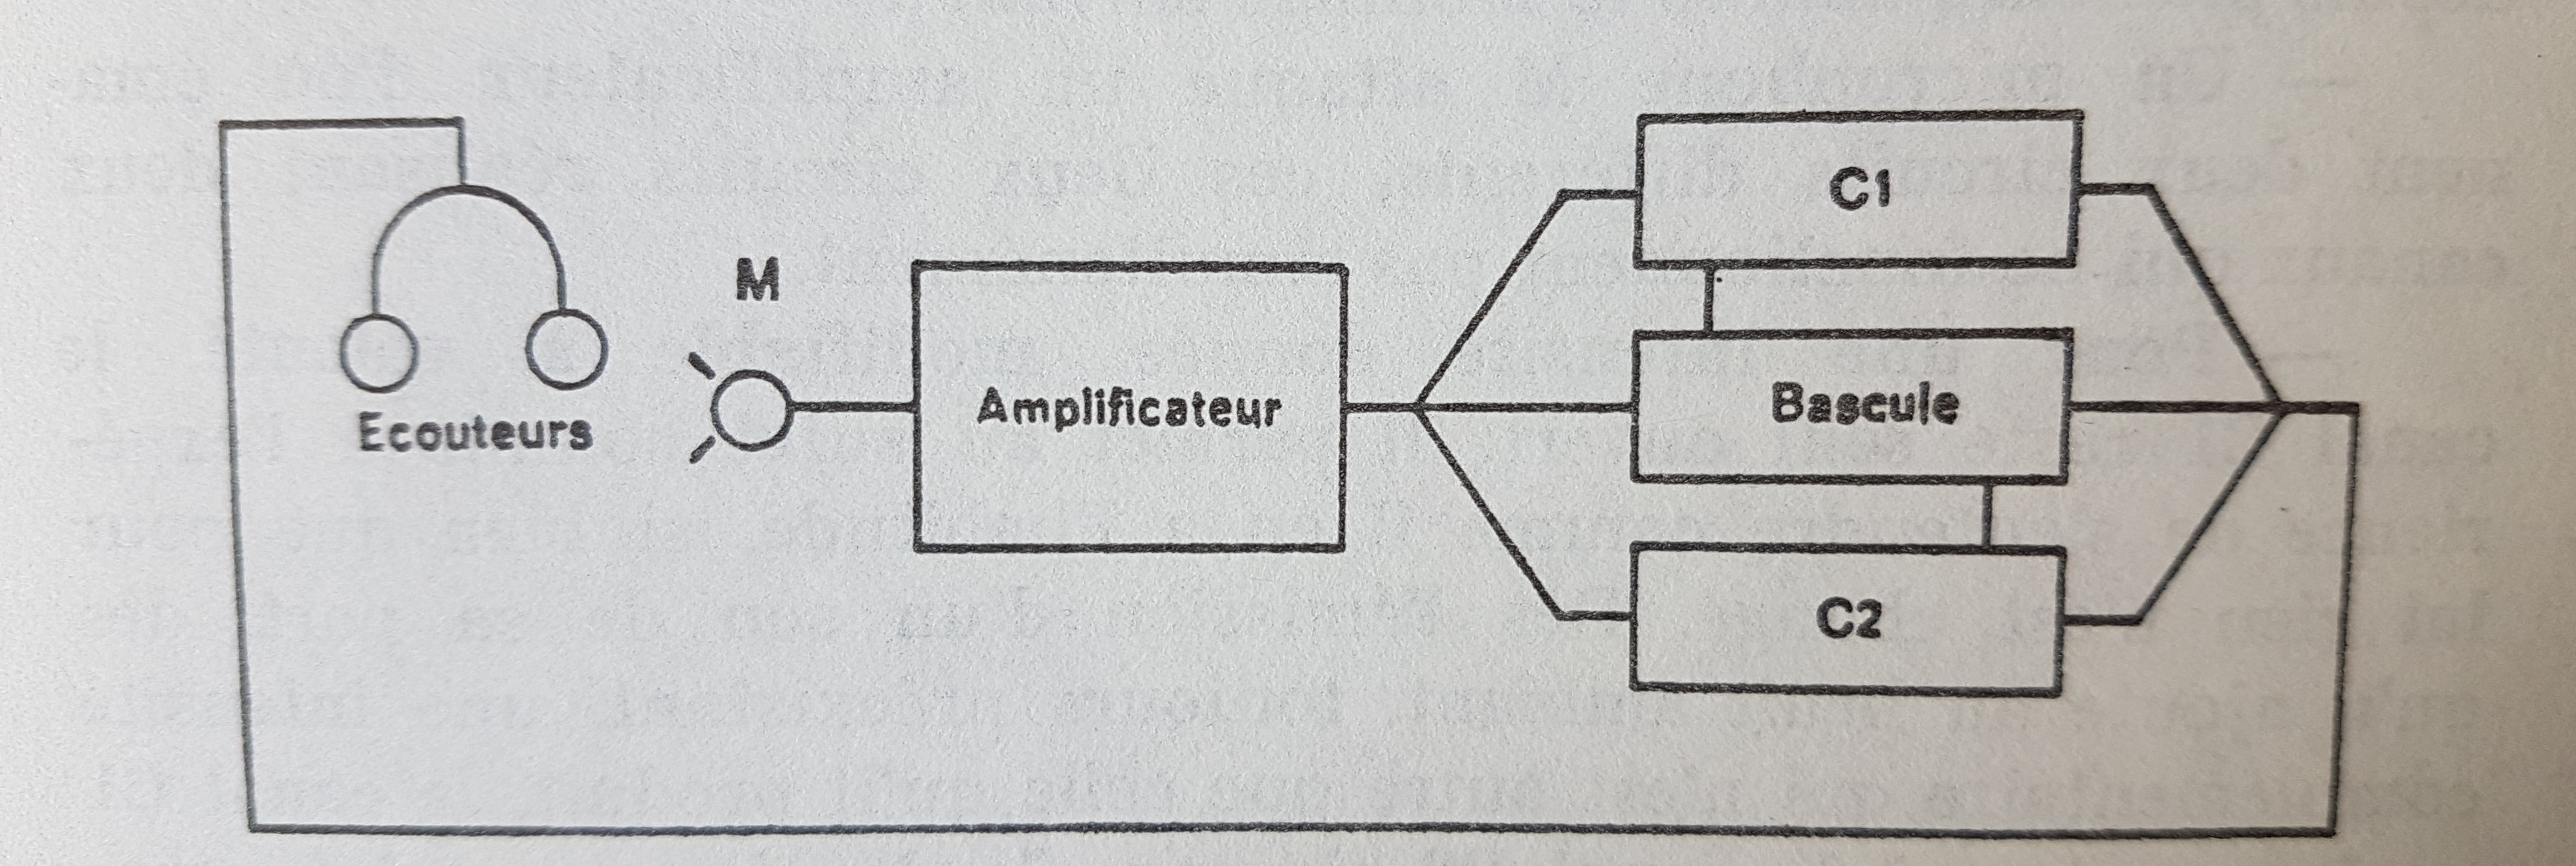
\includegraphics[width=0.7\linewidth]{images/oreilleelectro.jpg}
	\caption[oreilleelectro]{Schéma initial de l'Oreille
          Electronique}

	\label{oreilleelectro}
\end{figure}
En fait, ce schéma comprend le\textit{ feed-back}, un des principes
cybernétiques lié au concept de l'\textit{homéostasie} tel
mentionné dans le dictionnaire de
psychologie \autocite[298]{doronparot}.
% \footnote{Doron et Parot, rétroaction;
  %feedback positif = il faut varier, f.négatif= ne rien faire,  feed-back, Doron/ Parot, .p177 : cybernétique. Concept de l'homéostasie, Cannon}
En effet, dès les premières
séances, Tomatis constate une amélioration temporaire de la voix, se
stabilisant avec l'entraînement, et établissant ainsi le
\textbf{lien frappant} entre\textbf{ l'écoute et
  l'émission vocale}.

Ainsi la façon d'émettre un son, le timbre de la voix et la fluidité
verbale figurent parmi les
éléments clairement significatifs que nous allons aborder plus loin, ayant opté pour
cette méthode de test.
